% options:
% thesis=B bachelor's thesis
% thesis=M master's thesis
% czech thesis in Czech language
% slovak thesis in Slovak language
% english thesis in English language
% hidelinks remove colour boxes around hyperlinks

\documentclass[thesis=B,czech]{FITthesis}[2012/06/26]

\usepackage[utf8]{inputenc} % LaTeX source encoded as UTF-8

\usepackage{graphicx} %graphics files inclusion
% \usepackage{amsmath} %advanced maths
% \usepackage{amssymb} %additional math symbols

\usepackage{dirtree} %directory tree visualisation


\usepackage{float}

\usepackage{listings}
\lstset{frame=lrbt,xleftmargin=\fboxsep,xrightmargin=-\fboxsep, showstringspaces=false}

% % list of acronyms
% \usepackage[acronym,nonumberlist,toc,numberedsection=autolabel]{glossaries}
% \iflanguage{czech}{\renewcommand*{\acronymname}{Seznam pou{\v z}it{\' y}ch zkratek}}{}
% \makeglossaries

\newcommand{\tg}{\mathop{\mathrm{tg}}} %cesky tangens
\newcommand{\cotg}{\mathop{\mathrm{cotg}}} %cesky cotangens

% % % % % % % % % % % % % % % % % % % % % % % % % % % % % % 
% ODTUD DAL VSE ZMENTE
% % % % % % % % % % % % % % % % % % % % % % % % % % % % % % 

\department{Katedra Softwarového inženýrství}
\title{Webový server pro poskytování dynamicky generovaných objektů ve formátech RDF}
\authorGN{Jan} %(křestní) jméno (jména) autora
\authorFN{Řasa} %příjmení autora
\authorWithDegrees{Jan Řasa} %jméno autora včetně současných akademických titulů
\supervisor{RNDr. Jakub Klímek, Ph.D.}
\acknowledgements{Chtěl bych poděkovat vedoucímu mé práce RNDr. Jakubu Klímkovi za odborné vedení, pomoc při zpracování této práce a cenné rady.
Dále bych chtěl také poděkovat svým rodičům a přátelům za podporu nejen při tvorbě této práce, ale po celou dobu studia.}
\abstractCS{Řada objektů na webu dat tvoří natolik velkou skupinu (až nekonečnou), že je není možné všechny 
perzistentně uložit a publikovat. Je nutné nabídnout server, který na základě požadavku klienta na daný 
objekt příslušná data dynamicky vygeneruje a odešle klientovi.


Tato práce se zabývá analýzou již existujících řešení, návrhem a implementací daného serveru včetně otestování základní funkcionality.
Server bude umožňovat uživateli definovat RDF (Resource Description Framework) objekty pro dynamické 
generování v několika formátech.
Návrh bude zohledňovat již zaběhlé technologie z oboru Linked Data, jako je například dotazovací 
jazyk SPARQL (Protocol and RDF Query Language). Server bude implementován v jazyce Java.}

\abstractEN{There are many objects on the web of data that make such a big group (almost infinite) that it's not possible to persist them all and publish them.
It's necessary to offer a web server that to the client's requests to the given objects dynamically generates the data and sends them back to the client.

The goal of this bachelor's thesis is an analysis of existing solutions, to design and implement this web server, including tests of the basic functionality.
Users of the web server will be able to define RDF (Resource Description Framework) objects for dynamically generating in the several formats.
The design will include popular technologies from Linked Data such as SPARQL language  (Protocol and RDF Query Language). The server will be implemented
in Java.
}

\placeForDeclarationOfAuthenticity{V~Praze}
\declarationOfAuthenticityOption{4} %volba Prohlášení (číslo 1-6)
\keywordsCS{sémantický web, web dat, Linked Data, RDF, dynamické generování, SPARQL, Java, webový server \newpage}

\keywordsEN{semantic web, web of data, Linked Data, RDF, dynamically generating, SPARQL, Java, web server}

\begin{document}

% \newacronym{CVUT}{{\v C}VUT}{{\v C}esk{\' e} vysok{\' e} u{\v c}en{\' i} technick{\' e} v Praze}
% \newacronym{FIT}{FIT}{Fakulta informa{\v c}n{\' i}ch technologi{\' i}}

\begin{introduction}
\paragraph{}
Při publikování dat na webu dat je vždy důležité zamyslet se nad tím, jak a kde budou tyto data uložena.
Způsobů je mnoho. Mezi ty nejzákladnější patří ukládání dat do různých databázových systémů, nebo pouze přímo na určené místo na disku.
Oba zmíněné způsoby a jim podobné mají ovšem jeden zásadní problém, a tím je kapacita uložiště.

Pro uložení většiny informací, se kterými se lze setkat na webu, jako jsou obrázky, zprávy, informace o počasí a mnoho dalších, se tato skutečnot nemusí příliš řešit.
Kapacita uložiští nám pro tyto informace většinou stačí. Nicméně existuje řada informací (dále také objektů), které tvoří natolik velkou skupinu (až nekonečnou),
že je není možné všechny perzistentně uložit a publikovat.

Dobrým příkladem jsou například časová data - konkrétní čas či časový interval. V kontextu Linked Data \cite{linked_data} se často odkazuje na časový objekt.
Ať už se jedná například o časy příjezdů autobusů, časy uvedené ve statistických údajích,
nebo o datum nějaké události, vždy je potřeba mít daný časový objekt nějakým způsobem uložen.

Existují ale kapacity na uložení každého takového objektu? Časových objektů je přeci nekonečně mnoho. Mohou odkazovat jak do minulosti, tak do budoucnosti.
A není potřeba se omezovat pouze na časové objekty. Jako další příklad může být informace o vztahu mezi lidmi, respektive mezi kterýmikoliv subjekty.
Tyto informace taktéž vyžadují ohromné kapacity uložiští.

Mnoho typů objektů ale spojuje fakt, že mají vždy stejnou strukturu a jen část informací se mění (například jen sekunda, hodina, \ldots).
A to je ideální příležitost pro to, aby se ukládání těchto objektů zaměnilo za dynamické generování. Pro vygenerování objektu stačí vždy použít stejnou strukturu
a jen dosadit potřebné informace tak, aby vznikl požadovaný objekt.

\end{introduction}

\chapter{Cíl práce}
Cílem této práce je navrhnout, implementovat a otestovat webový server pro poskytování dynamicky generovaných objektů v RDF formátech.
Server bude splňovat následující požadavky:

 \begin{itemize}
  \item Server bude umožňovat administrátorovi založit nový typ objektů včetně jejich atributů a umožní nakonfigurovat URL, pod kterými budou objekty dostupné. 
  \item Typy objektů bude možné založit přes konfigurační soubor. 
  \item Klient bude moci přístupem na dané URL získat data o příslušném objektu. 
  \item Data o objektech budou klientům dostupná v RDF serializacích (RDF/XML, Turtle, N-Triples, JSON-LD) a jako webová stránka.
  \item Server bude využívat mechanismu Content Negotiation pro určení formátu výstupu požadavku klienta. 
  \item Server bude implementován v jazyce Java.
 \end{itemize}
\chapter{Analýza}

\section{Účel aplikace}
Webový server bude poskytovat uživatelům funkci pro dynamické generování objektů ve formátech RDF.
Uživatel si bude moci nadefinovat vlastní typy objektů pomocí šablony včetně URL, na které budou dané objekty přístupné.
Objekty budou generovány za použití informací, které bude obsahovat URL adresa při požadavku na daný objekt.

Tento způsob generování objektů ve velké míře šetří především finanční zdroje za pořizování nových uložišť. Pro velké množství stejných objektů (až nekonečně mnoho)
stačí vytvořit pouze jednu definici (šablonu) objektu, která se dle specifikovaných pravidel vyplní informacemi z URL adresy a uživateli se zobrazí jako 
požadovaný objekt.

Další výhodou je z hlediska jednotné definice objektů i možnost lehce upravit strukturu konkrétních definic na jednom místě.
Na konkrétní definici objektu může být odkazováno s různými parametry z mnoha jiných objektů a jedinou změnou v definici lze ovlivnit informace i v těchto objektech.
Měnit již dříve vytvořené a uložené konkrétní objekty v takovém počtu by bylo téměř nereálné.

Účelem serveru je také chování, které co nejméně omezuje možné klienty \footnote{Zde se klientem rozumí především aplikace které by k objektům přistupovaly.}.
Server využívá principu Content Negotiation \cite{content_negotiation} a podporuje nejpoužívanější typy RDF serializací, včetně možnosti zobrazit informace 
o objektu v HTML podobě při zobrazení prohlížečem.


\section{Existující řešení}
Pro funkce, které má tento server splňovat, neexistuje v současnosti žádné jiné řešení. Minimálně není možné dohledat 
  žádné veřejné řešení, ani informace o nějakém soukromém řešení, které by sloužilo například pro soukromá data v rámci nějaké společnosti. 
  Nicméně existuje velmi populární řešení jednoho typu objektu - časových intervalů, tzv. British Time Intervals, které je hojně používané,
  převážně pak také v rámci dat, které poskytuje britská vláda.
  
\subsection{British Time Intervals}
Pro popis těchto objektů je asi nejlepší odkázat se na konkrétní definici na webové stránce, ze které jsou tyto intervaly dostupné.\cite{british_ti}
\begin{quote}
 Linked data for every time interval and instant into the past and future, from years down to seconds.
 This is an infinite set of linked data. It includes government years and properly handles the transition to the Gregorian calendar within the UK.
\end{quote}
 Zde je vhodné všimnout si hlavně slov \textit{infinite set}, což přesně charakterizuje typy objektů, kterými se tato práce zabývá.

 \subsubsection{Struktura URI} Pro přístup k jednotlivým generovaným objektům slouží URL adresa, která má vždy předepsanou strukturu. Informace, které jsou dostupné
k tomuto datasetu, obsahují popis těchto struktur a jsou veřejně dostupné na stránkách společnosti Epimorphics \cite{ti_structure}. Takovou URL adresou může být například 
\textit{http://reference.data.gov.uk/doc/government-year/\{year1\}-\{year2\}}, kde po dosazení let míto \textit{year1} a \textit{year2} a přístupem na danou adresu získáme požadovaný 
objekt časového intervalu.

\subsubsection{Generování objektu} Takový objekt je tedy dynamicky vygenerován s použitím parametrů z URL adresy. Konkrétní popis toho, jak jsou tyto objekty interně generovány 
není veřejný, ale je velmi pravděpodobné, že je použit minimálně jeden z následujících způsobů:
\begin{itemize}
  \item Předem připravená RDF šablona (v libovolném formátu - Turtle, RDF/XML, N-TRIPLES \ldots) s placeholdery, do kterých se dosadí parametry z URL adresy.
  \item SPARQL \cite{sparql_w3c}\cite{sparql_bob} dotaz s placeholdery.
 \end{itemize}

 

\section{Požadavky}

\subsection{Funkční požadavky}
 \begin{itemize}
  \item přístup k administraci objektů přes více rozhraní
  \item podpora více formátů pro definice a zobrazení objektů
  \item zobrazení existujících definic objektů
  \item administrace definic objektů  
  \item konfigurace objektů bude možná několika způsoby
  \item vygenerování a zobrazení konkrétních objektů
 \end{itemize}
 
 \subsubsection{Přístup k administraci objektů přes více rozhraní}
 Administrátori bude umožněn přístup k definicím objektů dvěma způsoby:
 \begin{itemize}
    \item přes webové rozhraní
    \item přes API
 \end{itemize}
 Oba tyto způsoby budou poskytovat stejnou funkcionalitu. Webovým rozhraním se myslí jednoduchá aplikace pro administraci objektů z webového prohlížeče.
 API bude sloužit k administraci z jiných potenciálních aplikací.
 
 \subsubsection{Podpora více formátů pro definice a zobrazení objektů}
 Server bude podporovat následující formáty pro definice objektů přes API:
 \begin{itemize}
    \item JSON formát
    \item RDF serializace TURTLE \cite{turtle_example}
 \end{itemize}
 Konkrétní vygenerované objekty budou klientům dostupné v těchto RDF serializacích:
 \begin{itemize}
    \item RDF/XML \cite{rdf_xml}
    \item JSON-LD \cite{rdf_json_ld}
    \item N-TRIPLES \cite{rdf_n_triples}
    \item TURTLE 
 \end{itemize}
 Každá definice objektů bude také umožňovat definovat HTML formát objektu pro zobrazení v prohlížeči.
 
 \subsubsection{Zobrazení existujících definic objektů}
  Ve webové aplikaci budou zobrazeny všechny aktuální definice objektů v tabulce s možností konkrétní definici upravit (tedy také zobrazit definici konkrétního objektu)
  nebo smazat přes tlačítka vedle každé definice.
  
  Přes API bude možné získat definice objektů ve dvou formátech:
  \begin{itemize}
    \item RDF serializace
    \item JSON formát
 \end{itemize}
  Konkrétní formát bude určen principem Content Negotiation. Získat půjde seznam všech definic a také konkrétní definice.
 
 \subsubsection{Administrace definic objektů}
  Administrátorovi bude umožněno přidávat nové definice, měnit a mazat již vytvořené definice. Tyto akce budou umožněny jak z webové aplikace, tak i přes API.
  Dále bude moci administrátor definovat objekt konfiguračním souborem v RDF serializaci TURTLE.
  
  
  \subsubsection{Konfigurace objektů bude možná několika způsoby}  
  \label{sec:object_types}
  Koknfigurací objektů se zde myslí možné způsoby jak a z čeho se bude generovat výsledný RDF objekt. Server bude podporovat
  následující způsoby:
  \begin{itemize}
    \item generování ze SPARQL šablony - CONSTRUCT dotaz \cite{sparql_bob}
      \subitem Vstupem bude SPARQL šablona CONSTRUCT dotazu s placeholdery \footnote{Placeholder: část šablony, která jasně identifikuje místo, 
      kam se dosadí parametry z URL adresy.}, za které se dosadí při požadavku na objekt hodnoty z URL adresy
      a provede se příkaz který vygeneruje objekt.
      
     \item generování ze SPARQL šablony - vzdálený CONSTRUCT nebo DESCRIBE dotaz \cite{sparql_bob}
      \subitem Vstupem bude SPARQL šablona jako v prvním případě. Navíc bude možné provést DESCRIBE dotaz. Rozdíl oproti prvnímu případu je v tom, že se 
      dotaz přepošle na zvolenou adresu SPARQL Endpointu \cite{sparql_bob}, zde se provede a klientovy je pak vrácen daný objekt.
      
    \item generování z RDF šablony
     \subitem Vstupem bude RDF šablona podporovaných serializací s placeholdery, za které se dosadí při požadavku na objekt hodnoty z URL adresy. 
     
     \item Proxy objekt
      \subitem Server bude umožňovat roli prostředníka při generování objektů. Požadavek na objekt se přepošle na jiný server a výsledek se přeloží
      klientovi dle požadované serializace. Tento způsob umožňuje generování objektů přes jiné aplikace.
 \end{itemize}
 
 
  
  \subsubsection{Vygenerování a zobrazení konkrétních objektů}  
  Klient bude moci přístupem na konkrétní URL adresu získat data o příslušném objektu. Typ RDF serializace nebo zobrazení HTML stránky se určí přes 
  Content Negotiation.

\subsection{Nefunkční požadavky}
\begin{itemize}
    \item server bude implementován v jazyce Java
    \item celá aplikace bude uložena ve WAR souboru pro zjednodušené nasazení
 \end{itemize}
 
 \chapter{Návrh}
 
 \section{Použité technologie}
 
 \subsection{Resource Description Framework (RDF)}
 Resource Description Framework je rodina specifikací, která se používá jako metoda pro modelování informací - objektů.
 Jedná se o model metadat, které popisují nějaké zdroje.
 
 Příkladem může být obyčejná webová stránka obsahující nějaké informace. Webové stránky se zaměřují především na uživatele.
 Důležité je, aby se uživateli stránky líbily a dbá se tedy hodně na design. Pokud jsou stránky přehledné, pak člověk nemívá problémy pochopit
 dané informace. Nicméně stroj (počítač, program) tyto informace sice zobrazí uživateli, ale samotné informace si interpretovat nedokáže.
 
 RDF model popisuje tedy způsoby, jakými docílit toho, že poskytované informace budou čitelné i pro stroje.
 
 Základní kostrou RDF modelu dat jsou takzvané $trojice$. Tyto trojice se skládají ze subjektu, predikátu a objektu.
 Trojice se může volně přeložit i do podoby, kde subjekt má nějakou vlastnost (predikát) s konkrétní hodnotou (objekt). Tedy všechny trojice, které mají
 stejný subjekt tento subjekt definují.
 
 Každý subjekt je identifikován nejčastěji přes URI. Bavíme-li se o datech na webu, tak zde může být URI klasická URL adresa, jak ji známe
 z běžného používání. Co se týče objektu (hodnoty), tak se může jednat o literál (řetězec, číslo apod.), ale hodnotou může být zase URI nějakého dalšího objektu.
 Dokonce i predikát může být objektem s vlastním URI. Tím, že se objekt skládá z dalších objektů, které jsou jednoznačně identifikovány pomocí URI, získáváme velkou výhodu
 tohoto modelu. Ve výsledku vzniká graf popisující tyto trojice, což je i pro stroje čitelná struktura.
 
 Samotné RDF popisuje pouze model. Pro uložení tohoto modelu je zapotřebí informace nějakým způsobem serializovat. Pro uložení RDF objektů se 
 používají nejčastěji tyto RDF serializace:
 \begin{itemize}
  \item RDF/XML
  \item Turtle
  \item N-Triples
  \item JSON-LD
 \end{itemize}
 
 Pro ukázku je zde příklad ve formátu Turtle, který je převzat z W3C specifikace \cite{turtle_example}.
 \begin{lstlisting}[language=C, basicstyle=\small]
@base <http://example.org/> .
@prefix rdf: <http://www.w3.org/1999/02/22-rdf-syntax-ns#> .
@prefix rdfs: <http://www.w3.org/2000/01/rdf-schema#> .
@prefix foaf: <http://xmlns.com/foaf/0.1/> .
@prefix rel: <http://www.perceive.net/schemas/relationship/> .

<#green-goblin>
    rel:enemyOf <#spiderman> ;
    a foaf:Person ;  # in the context of the Marvel universe
    foaf:name "Green Goblin" .

<#spiderman>
    rel:enemyOf <#green-goblin> ;
    a foaf:Person ;
    foaf:name "Spiderman".
\end{lstlisting}
<$\#green-goblin$> je zde subjekt identifikovaný URI (http://example.org/\#green-goblin),
$rel$:$enemyOf$ je predikát - v tomto případě zase objekt identifikovaný URI (http://www.perceive.net/schemas/relationship/enemyOf) a 
 <$\#spiderman$> je objekt - zase identifikován URI.
 Tento model dohromady poskytuje informaci, že objekt na dané URI je nepřítelem Spidermana. $a foaf$:$Person$ znamená, že
 se jedná o objekt Person a $foaf:name "Green Goblin"$ zase to, že jeho jméno je Green Goblin. Tímto je tedy definován objekt $<\#green-goblin>$ a podobně tomu je u 
 objektu <$\#spiderman$>.
 
 \subsection{Linked Data}
  Linked data, jak už název napovdá, popisuje metodu propojování informací na webu dat mezi sebou.  
  Tim Berners-Lee popisuje Linked Data výstižně takto: 
  \uv{\textit{Semantic Web isn't just about putting data on the web. It is about making links, so that a person or machine can explore the web of data. 
  With linked data, when you have some of it, you can find other, related, data.}} \cite{TimBL_LD}
  
  Aby se publikovaná data mohly využívat v co největší míře, nestačí je pouze zpřístupnit na webu dat. Největší užitek přináší linkování těchto dat dohromady.
  Stejně, jak je tomu u HTML dokumentů, slouží pro linkování v rámci RDF URI, které jasně identifikují objekty. Nad takto prolinkovanými daty se poté dají
  najít různé vztahy, které by bez prolinkování nebylo monžé nalézt.
  
  Linked Data staví na těchto čtyřech základních principech:
  \begin{itemize}
   \item Pro názvy a identifikaci objektů se používá URI
   \item Aby byly data přístupné, používají se HTTP URI
   \item Při přístupu na konkrétní URI lze získat informace dle standardů RDF, SPARQL, \ldots
   \item Na ostatní data se odkazuje také přes HTTP URI
  \end{itemize}
  
  Při zohlednění všech těchto principů lze získat maximálně propojené informace a jak už bylo u RDF zmíněno, ve výsledku vznikne ohromný graf vzájemně
  propojených informací, ve kterém je možné následně najít cenné informace i o objektech, které na první pohled nemusí mít mezi sebou nic společného.

  
  \subsection{Java}
   Při vývoji je použit programovací jazyk Java. Použití javy vychází už z požadavků ze zadání. Hlavní důvody, proč je zde java vhodná a proč byla
   i jedním z požadavků jsou následující:
   \begin{itemize}
    \item Rozšířenost javy ve světě Linked Data
    \item Snadná integrace kvalitních knihoven pro práci s RDF
    \item Jednoduše nasaditelná aplikace přes webový archiv (war soubor)
    \item Výkon
   \end{itemize}
   Rozšířenost javy ve světě Linked Data je opravdu velká. Důvodem, proč je tento fakt zmíněn ve výhodách, je možnost případné snadné integrace dalších systémů
   pro vývojáře z tohoto oboru. Důležitým důvodem je zmíněný výkon aplikace. Na ten mají vliv jak knihovny pro práci s RDF, tak ale i samotný typ aplikace.
   Server si může uchovávat předzpracované šablony, patterny regulárních výrazů a další informace přímo v paměti, tudíž klient ve výsledku dostane výsledek rychleji,
   než by tomu bylo při použití například PHP nebo podobných jazyků.
   
   \subsection{Apache Jena}
   Pro práci s RDF daty byla zvolena knihovna Apache Jena. Tato knihovna podporuje práci přímo s RDF serializacemi a díky procesoru ARQ také práci se SPARQL
   dotazy. Další možností pro použití byla knihovna Sesame. Knihovny si jsou velice podobné. Obě mají dobrou dokumentaci i velmi dobře zpracované 
   ukázky, jak lze knihovny využívat. Rozhodujícím faktorem při výběru byl výkon.
   
   Při výkonostním srovnání byl zohledněn publikovaný test \textit{The Berlin\\ SPARQL Benchmark} \cite{sparql_benchmark}.
   Jena a Sesame se dle něj výkonostně velmi liší. Sesame je několikanásobně rychlejší na dotazování, ale Jena naopak s velkým náskokem vede při načítání souborů
   v Turtle formátu.
   
   Výkonostně má vliv načítání definic objektů, které se uchovávají v turtle formátu. Jedná se o proces, který bude spuštěn při zapnutí aplikace a při
   případném novém načtení (reloadu) definic (v případě nahrání definice přímo do filesystému dle požadavku). Rychlost SPARQL dotazů tedy není v tomto
   případě tolik důležitá. Při požadavku klienta na vygenerování objektu už se s RDF definicí nijak nepracuje - není potřeba se nad definicemi dále dotazovat.
   U typů SPARQL Endpoint/Construct také nedocházi k dotazovaní se nad lokálně uloženými daty.
   
   \subsection{Další Java knihovny}
   \begin{itemize}
    \item Jersey, GSON - pro práci s definicemi objektů v rámci API
    \item Log4j - logovací systém
    \item Typesafe - konfigurace
    \item JUnit - testování
   \end{itemize}
   
   \subsection{Maven}
   Závislosti, sestavení a testování se provádí přes build manažer Maven. Maven byl vybrán jako standard pro většinu Java aplikací.
   Vývoj taktéž probíhal v IDE IntelliJ IDEA, které obsahuje velmi dobrou integraci tohoto systému.
   
   \subsection{AngularJS}
   Součástí celého systému je i webová aplikace pro správu definic objektů. Zde je použit framework AngularJS, který je snadno napojitelný
   na REST API serveru. 

   \newpage
   
 \section{Návrh architektury}
  Na diagramu \ref{parts} lze vidět, že je systém rozdělen do 2 částí. První částí je webová aplikace, která slouží pro ulehčení administrace definic objektů.
  Hlavní funkcionalita tohoto serveru ale není touto částí ovlivněna, na API se lze napojit i z jiných aplikací.
  Tato část je napsaná ve frameworku AngularJS která využívá serverové API.
  U této aplikace se dá mluvit o známé MVC\footnote{Model-View-Controller} architektuře, kde je ovšem Model (zde definice objektu)
  primárně součástí druhé části systému.
  
  Druhou částí je serverová část, dále také pod názvem \textit{Jádro systému}. Architektura této části je velice podobná MVC architektuře. O čistém MVC nelze 
  mluvit z toho důvodu, že je zde velká provázanost komponent a není až tak striktně oddělena zodpovědnost jednotlivých částí.
  
  \begin{figure}\centering
 	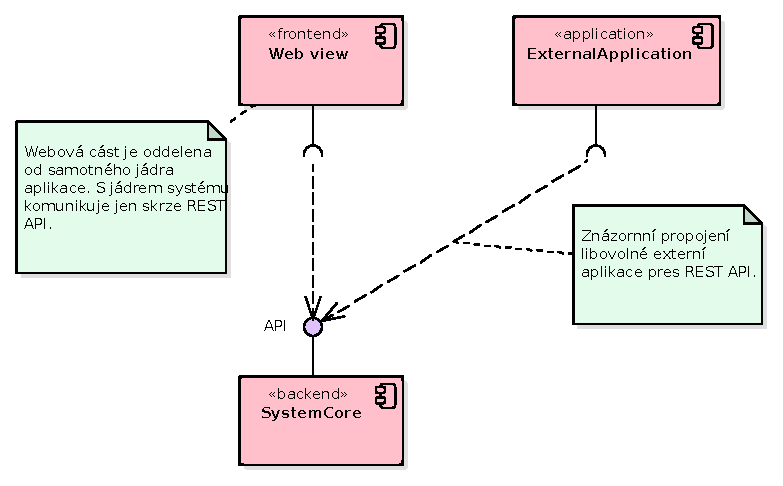
\includegraphics[width=1\textwidth]{Component_Model.pdf}
 	\caption[Základní části systému]{Diagram zobrazuje dvě základní části systému (jádro systému a webová, nebo jakákoliv jiná aplikace napojená na API)}\label{parts}
 \end{figure}
  
  \subsection{Jádro systému}  
  Jádro systému se skládá ze čtyř hlavních komponent, které lze také vidět na obrázku \ref{packages_core}. Pro administraci definic objektů slouží komponenta API. Další komponentou je Model, který obsahuje
  třídy využívané všemi komponentami. O načítání, ukládání a přístup k definicím objektů se stará komponenta Container.
  Poslední základní komponentou je Publisher, který zpřístupňuje celý systém klientovi v podobě vygenerovaných objektů.
  
  
  \begin{figure}\centering
 	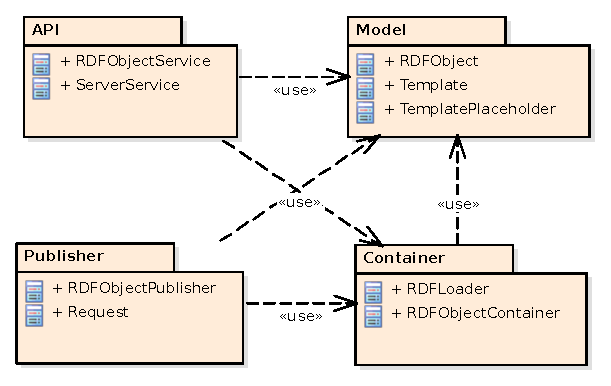
\includegraphics[width=0.8\textwidth]{Components.pdf}
 	\caption[Model komponent]{Základní čtyři komponenty jádra systému}\label{packages_core}
 \end{figure}
  
  \subsubsection{Komponenta API}
    Tato komponenta slouží pro administraci definic objektů. Jedná se o komponentu, ke které má přístup pouze administrátor systému. Obsahuje dvě třídy, které
    mají své metody vystavené pro napojení přes API.
    
    Tyto třídy jsou zobrazeny na obrázku \ref{api_class}. Třída RDFObjectService slouží k samotnému vytváření, úpravě a mazání definic. ServerService pak obsahuje
    metodu, která se dá taktéž volat přes API a slouží ke znovunačtení všech definic z nastaveného uložiště.
    \begin{figure}\centering
 	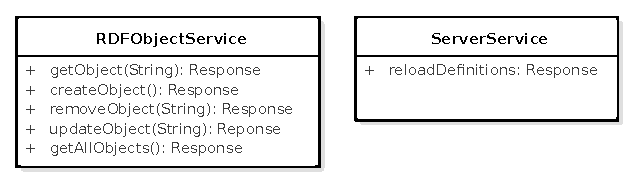
\includegraphics[width=0.8\textwidth]{API.pdf}
 	\caption[Model tříd API]{Třídy reprezentují služby, které mají metody vystavené pro API}\label{api_class}
    \end{figure}
    
    \subsubsection{Komponenta Model}
    Tato komponenta obsahuje tři základní třídy, které jsou využívány zbytkem aplikace. Jedná se o třídy RDFObject, Template a TemplatePlaceholder, které jsou zobrazeny
    na obrázku \ref{model_class}.
    
     \begin{figure}\centering
	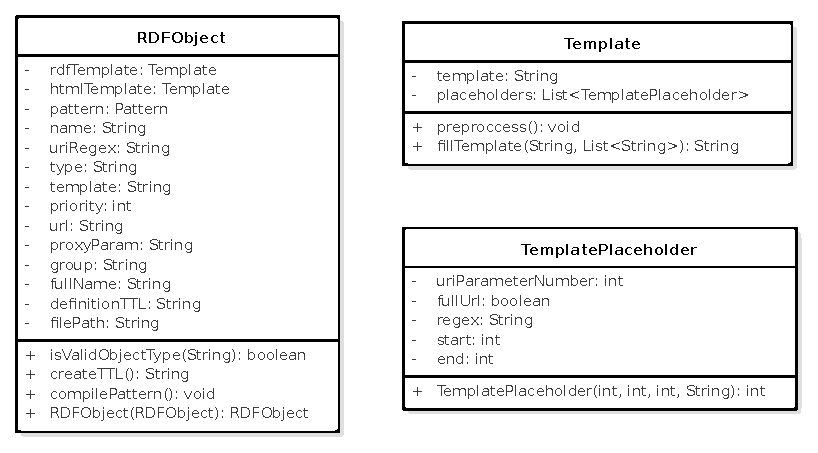
\includegraphics[width=\textwidth]{Model.pdf}
	\caption[Model tříd komponenty model]{Třídy v komponentě Model. Pro přehled jsou uvedeny pouze nejdůležitější metody. Třídy jinak obsahují i další metody, převážně settery a gettery.}\label{model_class}
    \end{figure}
    
    RDFObject reprezentuje samotnou definici objektu. Obsahuje dva atributy typu Template. Prvním z nich je šablona definice (RDF serializace, nebo SPARQL dotaz) a
    druhou je HTML šablona sloužící pro zobrazení objektu v HTML formátu. Dále obsahuje metody jako jsou například validace a kompilace patternu
    regulárního výrazu pro pozdější identifikace definice dle požadavku klienta. Obsahuje také gettery a settery pro atributy, které ale nejsou
    na zmíněném diagramu vidět pro jejich primitivnost.
    
    Třídy Template a TemplatePlaceholder zastřešují celý šablonovací systém. Třída Template obsahuje dvě důležité metody pro přdzpracování šablony
    a následné vyplnění šablony při požadavku. Předzpracování šablony probíhá tak, že se v šabloně naleznou všechny placeholdery a uloží se do seznamu
    pro pozdější vyplnění. Předzpracování probíhá pouze jendou při nahrátí definic (při startu serveru nebo znovunačtení definic). Cílem takto
    předzpracované šablony je urychlení generování objektů tak, aby se pouze dosazovaly hodnoty a případně aplikovaly podporované regulární výrazy.
 
 \subsubsection{Komponenta Container}
 O správu nahraných definic se stará komponenta Container. Z obrázku \ref{container_class} je patrné, že obsahuje 2 třídy.
 
 Třída RDFLoader se stará
 o čtení jednotlivých definic z file systému a následnou transformaci definice v Turtle formátu do objektu RDFObject,
 který reprezentuje konkrétní definice.
 
 Třída RDFContainer slouží jako kontejner (malá databáze) všech nahraných objektů. Objekty si drží jak podle celého jména definice pro rychlý přístup
 k definicím pro API, tak i podle priorit, podle kterých dochází k vyhledávání definic při požadavku klienta.
 Kontejner se v aplikaci vyskytuje díky použití singleton patternu
 pouze jeden a je nejvytíženějším objektem v celé aplikaci, protože je využíván všemi komponentami.
 
 \begin{figure}\centering
 	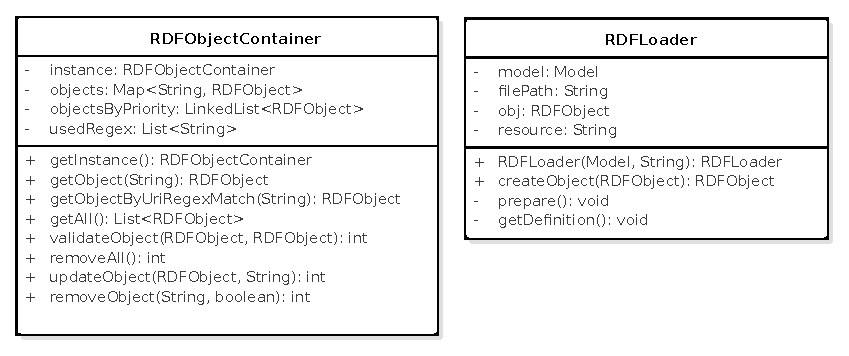
\includegraphics[width=\textwidth]{Container.pdf}
 	\caption[Model tříd komponenty container]{Komponenta container obsahuje třídy pro administraci objektů}\label{container_class}
    \end{figure}
    
    \subsubsection{Komponenta Publisher}
    Tato komponenta slouží k odbavování požadavků klienta na vygenerování objektu. Na obrázku \ref{publisher_class} lze vidět 2 třídy,
    které mají za úkol interakci s klientem.
    
    Třída RDFObjectPublisherService zpracovává prvotní požadavek klienta metodou $handleObjectRequest()$. V rámci systému je tato metoda definována
    pro všechny podporované serializace výstupu (HTML, RDF/XML, Turtle, JSON-LD a N-Triples). Při zavolání těchto metod je dále vytvořen 
    objekt třídy Request, kterému je předána zodpovědnost za vygenerování výsledného objektu. 
    
    \begin{figure}\centering
 	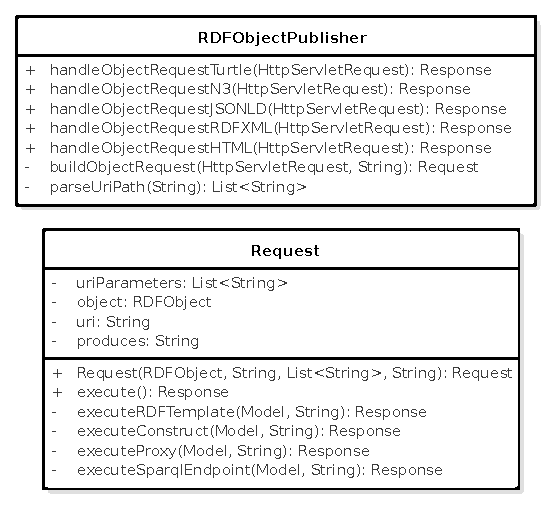
\includegraphics[width=0.8\textwidth]{Publisher.pdf}
 	\caption[Model tříd komponenty publisher]{Komponenta publisher obsahuje třídy pro zpracování požadavků klienta}\label{publisher_class}
    \end{figure}
    
    
   \newpage
   
   
 
 \section{Identifikace objektů, URL}
 \label{sec:identifikace}
 V kontextu RDF se dají objekty identifikovat pouze jedním způsobem, a to URL adresou. V tomto případě ale URL zastává ještě jednu důležitou úlohu.
 Vzhledem k tomu, že je jediným spojením mezi objektem (a jeho definicí) a vnějším prostředím, tak musí nést i informace, ze kterých bude později vygenerován
 konkrétní objekt. Návrhu struktury URL byla proto věnována velká pozornost.
 
 \subsection{Struktura URL v.1}
 Prvotní návrh byl takový, že se URL rozdělí na následující 3 části:
 \begin{itemize}
  \item Hostname
   \subitem Touto částí se rozumí identifikace serveru a protokolu, například \textit{https://dynrdf.com}. Z pohledu objektu slouží jen jako část identifikátoru.

    \item Identifikace objektu - první část cesty za hostname
     \subitem Tato část slouží k identifikaci objektu. Jedná se o unikátní název pro každý objekt. Příkladem může být například objekt časového intervalu s URL začínající 
     \textit{https://dynrdf.com/time-interval}, kde \textit{time-interval} identifikuje tento objekt.
     
    \item Parametry objektu
     \subitem Zbývající část URL nese informace, které se dosadí do šablon jednotlivých definic objektů. Jednotlivé parametry jsou vždy odděleny lomítkem.
     Například pro objekt ročního intervalu by mohla URL vypadat následovně \textit{https://dynrdf.com/time-interval/2015/2016}, kde by zvolené roky znamenaly 
     parametry \textit{od} a \textit{do}.
 \end{itemize}
 Tento návrh by byl naprosto dostačujícím pro generování objektů všech podporovaných typů. Nicméně s sebou nese dva velké problémy.
 
 Prvním problémem je ten, že by musel být každý objekt identifikován IP adresou nebo doménou, kde tento server bude spuštěn. To by tedy znamenalo, že
 by tu nebyla možnost určit pro každý objekt extra URL v identifikátoru. Pokud by například funkce tohoto serveru chtěly využívat dvě různé společnosti, které
 by svoje objekty dále publikovali, tak by mohlo docházet k nekonzistenci odkazů na objekty. Jinými slovy se dá také zeptat na to, proč by nějaká společnost chtěla 
 publikovat data, kde jejich identifikace není spojena například s názvem společnosti. Vždy by v identifikaci figuroval tento server, který ale s původem dat nemá
 nic společného. Cílem tohoto systému je pouze generovat objekty a identifikaci a vlastnictví ponechat na autorovi daných definic objektů.
 
 Druhý problém, nebo spíše nepříjemnost nastavá v případě, že by se servery společností využívající tohoto dynamického generování chovali jako prostředníci 
 a požadavky na objekty přeposílaly na tento server. Pokud by každá definice měla vždy konkrétní unikátní identifikátor v URL adrese, pak by se pro každý takový objekt 
 muselo přidávat pravidlo ve webových serverech na přeposílání požadavku a případně i dál složitě parsovat URL z požadavku na primárním serveru na URL, která by byla 
 dle zmíněných specifikací.
 
 Pro lepší představu, jak může vypadat požadavek na konkrétní objekt přes prostředníka, třetí stranu, slouží obrázek \ref{request_flow_2}. Při požadavku
 přímo na tento server z klienta se proces na jiném serveru přeskočí. Ani jeden z těchto způsobů právě není bez nějakého výše zmíněného problému. 
 \begin{figure}\centering
 	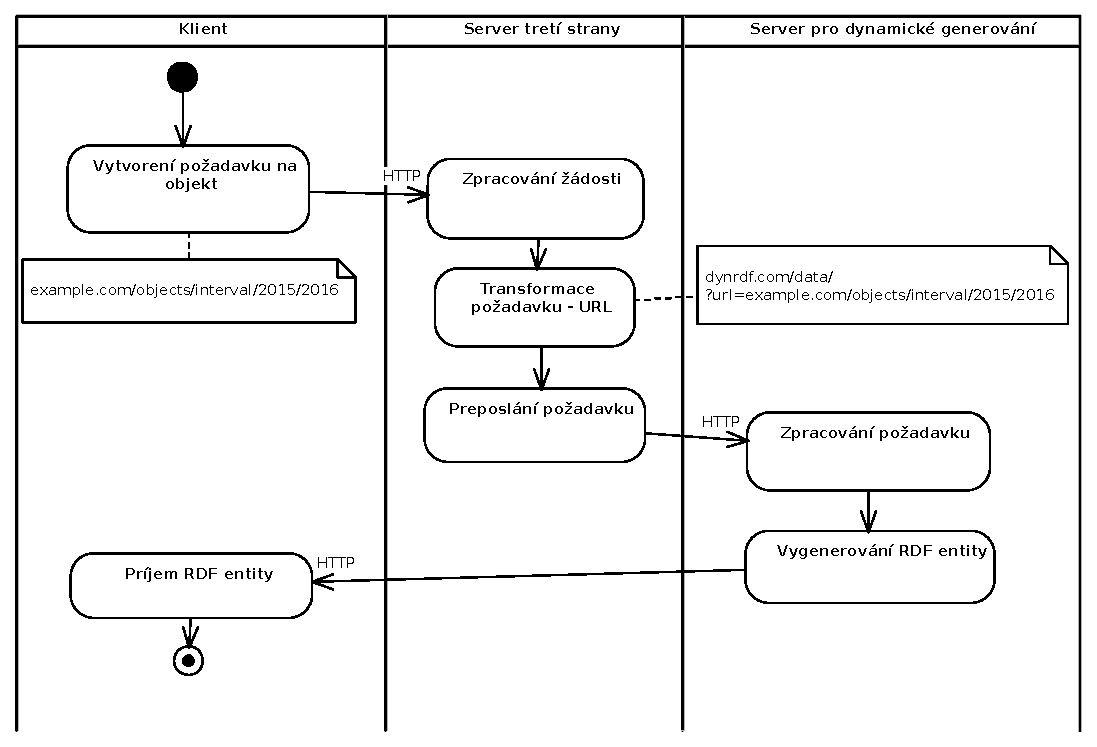
\includegraphics[width=1\textwidth]{request_flow}
 	\caption[Požadavek na objekt přes server třetí strany]{Požadavek na objekt přes server třetí strany. Prvotní návrh struktury URL adresy.}\label{request_flow_2}
 \end{figure}
 
 \subsection{Struktura URL v.2}
  Výše zmíněný návrh by znamenal téměř nepoužitelnost tohoto systému. Bylo proto nutné navrhnout jiné řešení. To se od původního návrhu liší na dvou místech, v předání
  informací o objektu a identifikací objektů.
  
  \subsubsection{Informace o objektu v GET parametru}
   Předání dat o objektu v GET parametru naprosto jednoduše řeší problém s parsováním URL adresy na serverech třetích stran. V případě, kdy na jiný server přijde požadavek
   na nějaký objekt, tak stačí v konfiguraci webových serverů nastavit pouze jedno pravidlo pro přeposlání požadavku pro všechny objekty.
  
  \subsubsection{Identifikace objektů, regulární výraz}
   Předání informací o objektu v GET parametru má ale za následek, že URL adresa už neobsahuje identifikátor objektu jako první část cesty. Objekt se dá identifikovat 
   pouze z informací v GET parametru, pro který účelově není stanovena žádná struktura.
   
   Strukturu URL adresy v GET parametru, která má identifikovat konkrétní objekt, zná pouze autor definice. Ideálním nástrojem, jak docílit mapování URL na konkrétní
   objekt je zde regulární výraz, který popisuje konkrétní strukturu požadavku.
   
\subsection{Shrnutí}
   Druhým návrhem struktury URL adresy se docílilo toho, že tento server bude schopný generovat objekty, jejichž identifikátor (URL) nebude závislý na adrese, kde tento
   server bude spuštěn.
   
   Příkladem může být například adresa \\ \textit{http://dynrdf.com/?url=http://dataowner.com/objects/year/2015}. Původní požadavek mohl přijít na server, 
   který je uveden v parametru \textit{url}. Tento požadavek byl následně přesměrován na tento server pouze pomocí jednoho pravidla, kde se za parametr dosadila 
   původní URL adresa požadavku. Následně se vygeneruje objekt roku 2015, jehož identifikátorem je obsah url parametru.

   \newpage
   
 \section{Definice objektů}\label{obj_def}
  Každý objekt, který má být dynamicky generován tímto systémem, musí být nadefinován administrátorem a následně uložen.
  Základními atributy, které daná definice musí obsahovat jsou:
  \begin{itemize}
    \item název
      \subitem Název slouží k identifikaci objektu v rámci seznamu.
    \item skupina
      \subitem Skupina zde označuje například název společnosti, jméno autora, nebo jiný identifikátor autora dané definice objektu. 
      Společně s názvem tvoří plně kvalifikované jméno definice.
    \item URL regex
      \subitem Tento regulární výraz slouží k identifikaci konkrétní definice.
    \item priorita objektu
      \subitem Priorita ovlivňuje pořadí definic, v jakém se pokouší systém najít shodu regulárního výrazu s příchozí URL. Některé regulární
      výrazy moho popisovat více objektů. Pokud je nějaký výraz více specifičtější než jiný, tak se zvýšením priority dané definice dosáhne k požadované shodě.
      Priorita se určuje celým číslem. Čím menší číslo, tím větší priorita a tím dříve se bude snažit systém najít shodu s příchozí adresou právě u dané definice.
      
    \item typ definice
      \subitem Typ definice označuje způsob zadání a vygenerování výsledného objektu. Konkrétním typům dle požadavku \ref{sec:object_types} se tento text věnuje dále.
    \item šablona objektu
      \subitem Šablonou se zde rozumí text vyplněný placeholdery, do kterých se při generování doplní hodnoty. Šablonou může být SPARQL dotaz nebo kterákoliv 
      podporovaná RDF serializace.
      
    \item HTML šablona
      \subitem Jedná se o podobnou šablonu jako pro konkrétní objekt, která je určena pro zobrazení ve webových prohlížečích.    
 \end{itemize}
 U některých typů jsou definovány výjimky, nebo další povinné atributy. Tyto specifikace jsou zmíněny dále u popisu těchto typů.
 
 Definice objektů přes Turtle formát musí splňovat RDF schéma, které je dostupné v příloženém souboru \textit{dynrdf.rdfs.ttl}.
 
 \subsection{RDF serializace}
   Definice objektu, který je definovám šablonou v RDF formátu, musí obsahovat všechny zmíněné povinné atributy. Do RDF šablony jsou doplněny při generování parametry z
   URL a vyplněná šablona je poté už výsledným požadovaným objektem.
 
 \subsection{SPARQL Construct}
  Šablonou pro tento typ je SPARQL construct dotaz, kde se jednotlivé parametry bindují pomocí funkce \textit{BIND()}. Tento typ definice díky jazyku 
  doplňuje RDF serializace o další funkcionality tohoto dotazovacího jazyka.
  
  Pro vygenerování objektu jsou zde zapotřebí 2 kroky. Dosazení parametrů do šablony jako v případě RDF serializace a následně spuštění SPARQL dotazu lokálně, který
  vytvoří požadovaný objekt.
  
 \subsection{SPARQL Endpoint}
  SPARQL je navržen pro dotazování se nad datasety. Tato data jsou dostupná přes služby běžící na SPARQL protokolu. Tento typ tedy slouží ke konstrukci
  komplikovanějších objektů, jejichž atributy mohou být výsledkem dalších SPARQL dotazů nad konkrétním datasetem. Výsledkem tohoto typu je RDF dokument construct
  nebo describe dotazu.
  
  Oproti lokálnímu construct dotazu se tento dotaz vykonává na jiném serveru. Proto je pro tento typ definice dalším povinným atributem URL adresa endpointu.
  
 \subsection{Proxy}
  Server má fungovat také jako prostředník mezi klientem a jinou aplikací poskytující RDF objekty. Jinou aplikací se rozumí webová služba, na kterou se bude požadavek
  přeposílávat. Tyto aplikace nemusí implementovat překlad objektů do jiných RDF serializací. Překlad do požadovaných serializací funguje zde na serveru stejně jako
  pro ostatní objekty.
  
  Pro tento typ definice není potřeba definovat šablonu objektu, ale dalšími povinnými atributy jsou:
  \begin{itemize}
  \item proxy URL
    \subitem Jedná se o URL webové služby pro předaní zodpovědnosti za vygenerován objektu.
    
  \item název GET parametru
    \subitem Příchozí URL s informacemi o objektu je také přeposlána na danou službu. Názvem GET paramteru se rozumí parametr, do kterého se dosadí tato URL.
 \end{itemize}
 
 \section{Šablonovací systém}
 Šablonovací systém je jedním ze stavebních kamenů této práce. Vyplněním šablony vzniká buď už konkrétní objekt, nebo SPARQL dotaz pro vygenerování objektu.
 Cílem návrhu tohoto systému je jednoduchost, ale zároveň dostatečná funkcionalita pro generování objektů různými způsoby.
 
 \subsection{Placeholder}
 Data o objektech jsou do šablon dosazeny přes placeholdery. Placeholderem se rozumí textový objekt, který definuje místo v dokumentu pro dosazení parametrů
 a má takovou strukturu, aby ho nebylo možné zaměnit s částí textu která nemá být nahrazena. V kontextu této práce se bude placeholderem rozumět textový objekt
 v tomto formátu:
 \begin{equation} \label{eq:placeholder}
 [@<d>[, <regex>]]
 \end{equation}
 
 Placeholder se skládá ze dvou částí. První povinnou částí je parametr \textit{@<d>}, který určuje konkrétní parametr URL adresy objektu,
 který se místo placeholderu dosadí. Jedná se tedy o \textit{vstup} do placeholderu.
 Druhým nepovinným parametrem je regulrní výraz, který se může aplikovat před dosazením textu na vstup placeholderu.
 
 \subsubsection{Vstup placeholderu}
 Jak bylo zmíněno v kapitole o identifikaci objektu \ref{sec:identifikace}, každý objekt je definován URL adresou, která je serveru předána GET parametrem.
 Pomocí informací, které obsahuje tato adresa, je potřeba vygenerovat konkrétní objekt.
 
 URL adresa je pro vstup do placeholderů rozdělena na části mezi lomítky. Na tyto části se dá odkazovat v placeholderu následujícím způsobem. Jako příklad 
 budou uvedeny reference k adrese \textit{http://intervals.com/year-interval/2013/2016}.
  
 \begin{itemize}
  \item @0 - reference na celou adresu\\(\textit{http://intervals.com/year-interval/2013/2016})
  \item @1, @2, \ldots (kladné čísla za znakem \textit{@}) jsou reference na pozice mezi lomítky URL adresy.
    \subitem @1 = \textit{http:}
    \subitem @2 = prázdný řetězec (mezi \textit{//})
    \subitem @3 = \textit{intervals.com}
    \subitem @4, @5, @6 postupně \textit{year-interval}, \textit{2013} a \textit{2016}
 \end{itemize}
 Tento způsob dává autorům šablon celkem snadný způsob, jak přímo z URL adresy dosadit do šablony požadované informace. Nicméně né všechny URL identifikátory objektů
 nemusí mít takovouto strukturu, aby se dalo snadno referencovat na konkrétní atributy objektu. Pokud by například v uvedeném příkladu nebyly roky rozděleny lomítkem,
 ale byly by v jednom parametru jako text \uv{\textit{2013-2016}}, nedal by se tento atribut rozdělit v RDF šabloně. Musel by se využít SPARQL construct dotaz, protože
 SPARQL obsahuje i funkce pro práci z řetězci (regulární výrazy). Proto je v placeholderu jako druhým nepovinným parametrem regulární výraz.
 
 \subsubsection{Regulární výraz v placeholderu}
  Pro možnost extrahování pouze části hodnoty parametru v šabloně slouží nepovinný atribut regulárního výrazu. Tento regulární výraz
  podporuje Capturing groups \cite{capture_group}. A to způsobem, kdy je ze vstupu placeholderu extrahována hodnota, která se nachází ve skupině číslo 1.
  
  Pokud by se autor šablony chtěl referencovat například na atribut \textit{@5} který by obsahoval\uv{\textit{2013-2016}}, 
  použil by jako placeholdery [@5, ``(\textbackslash d+)-''] pro \textit{2013}, resp. [@5, ``-(\textbackslash d+)''] pro \textit{2016}.
  Autoři šablon nebudou tedy nuceni používat SPARQL pro případy, kdy by potřebovali získat pouze část atributu, případně část z celé URL.
  
  \section{API}
  API je další důležitou komponentou v aplikaci. Slouží pro ulehčení administrace definic a zároveň otevírá možnosti pro napojení externích
  aplikací do systému. 
  
  Prvotním návrhem API bylo pouze několik funkcí, které by zpracovávaly požadavky v JSON formátu pro základní CRUD
  operace. Vzhledem ale k tomu, že celá aplikace pracuje primárně v RDF formátech, byly tyto funkce rozšířeny i o další, které umožňují administraci
  objektů za pomoci definic v Turtle formátu. Jedná se o totožné soubory, které administrátor může nahrát do složky s definicemi objektů, odkud se 
  při startu nebo reloadu aplikace nahrají do systému. Výhodou tohoto kroku je i validace při požadavku na vytvoření nebo aktualizaci definice,
  která se u definic přímo vložených do složky provádí až při dalším spuštění nebo reloadu. Administrátor tedy může vidět chyby nebo možné konflikty
  ihned při pokusu o nahrátí definice přes API a nemusí hledat v logu důvody, přoč byla jeho definice, kterou nahrál přímo do složky, odmítnuta.
  
  Celé API je rozdělené do dvou částí. Tou první je část pro zmíněnou administraci objektů, druhou pak API pro operace nad celým systémem.
  Nyní se počítá u systémového API pouze s funkcí pro znovunačtení definic ze složky pro ně určené. Pro tuto jedinou funkci by se API rozdělovat nemuselo,
  nicméně se počítá s dalším vývojem, kdy může být zapotřebí spravovat již běžící instanci serveru. Pro tyto operace už je vhodné rozdělit API na dvě části.
  
  \subsection{Struktura API}
  Pro administraci definic se v API využívá několik základních typů HTTP požadavků. Všechny operace také podporují vstup, respektive výstup v několika
  formátech. Stejně jako při požadavku klienta na konrétní objekt je zde využito principu Content negotiation.
  
  \subsubsection{Vytvoření objektu}
  Vytvoření objektu je možné jak ve formátu JSON, tak i v Turtle. Při vytváření objektu dochází také k validaci definice.
  Výsledek operace se klient dozví přes kód odpovědi (200 - úspěch, 400 - chyba). V případě neúspěchu je v odpovědi k dispozici i popis chyby.
  Parametry HTTP požadavku jsou následující:
  \begin{itemize}
   \item Cesta: /api/objects
   \item Typ požadavku: POST
   \item Content type: application/json, text/turtle
  \end{itemize}
  
  \subsubsection{Aktualizace objektu}
  Stejně jako při vytváření objektu je i změna objektu možná přes JSON i Turtle a provádí se také validace.
  Zde jsou parametry HTTP požadavku následující:
  \begin{itemize}
   \item Cesta: /api/objects/<fullname>
    \subitem <fullname> zde označuje řetězec ve formátu <skupina>/<název> (parametry definice)
   \item Typ požadavku: PUT
   \item Content type: application/json, text/turtle
  \end{itemize}

  \subsubsection{Smazání objektu}
  Parametry požadavku pro smazání jsou:
  \begin{itemize}
   \item Cesta: /api/objects/<fullname>
   \item Typ požadavku: DELETE
  \end{itemize}
  
  \subsubsection{Přístup k definicím}
  Klient si přes API může nechat zobrazit definici konkrétního objektu nebo celou sadu definic. Pro zobrazení si může také
  vybrat jakýkoliv z podporovaných formátů.
  Struktura požadavku je následující:
  \begin{itemize}
   \item Cesta: /api/objects/[<fullname>]
    \subitem Pokud chce uživatel získat konkrétní definici, tak za nepovinný parametr <fullname> dosadí stejně jako například u vytváření objektu
    celé jméno ve tvaru <skupina>/<název>. Pro zobrazení všech definic se tento parametr vynechá.
   \item Typ požadavku: GET
   \item Content type: libovolný z podporovaných (například text/turtle, application/n-triples \ldots)
  \end{itemize}
  
  \subsection{RDF schéma}
  Každá definice objektu má povinné atributy, které musí obsahovat. Pro popis těchto atributů, respektive celé definice, slouží RDF schéma (RDFS).
  RDF schéma je rozšířením RDF umožňující popsat konkrétní zdroje. V kontextu této aplikace se jedná o definice objektů.
  
  RDFS této aplikace popisuje definice jako objekty tříd konkrétních typů definic (RDF serializace, Sparql Construct \ldots). Dále definuje atributy, jako jsou
  například \textit{dynrdf:priority} nebo \textit{dynrdf:regex}. Pokud autor neví, k čemu například tyto atributy slouží, může se podívat 
  do schématu a přečíst si například komentář ke konkrétnímu atributu. Schéma k definicím je možné zobrazit si v příloze pod názvem $dynrdf.rdfs.ttl$.
  
  
  
  \chapter{Implementace}
  Implementace probíhala už také zčásti při analýze. Bylo potřeba připravit si celý projekt, převážně pak vyzkoušet a osvojit si práci s knihovnami
  pro RDF (Apache Jena) a tvorbu webových služeb v Javě. Jako vývojové prostředí bylo po předchozích zkušenostech zvoneno IntelliJ IDEA od společnosti 
  JetBrains.
  Při implementaci byl zohledněn následující vývojový plán:
  \begin{itemize}
   \item Vytvoření prototypu webové služby a deploy na Glassfish \cite{glassfish}
   \item Tvorba modelu definic a persistence
   \item API a webové rozhraní
   \item Vývoj šablonovacího systému
   \item Zpracování požadavku klienta a vygenerování výsledného objektu
  \end{itemize}
  
  
  \section{Prototyp webové služby}
  Cílem vývoje prototypu webové služby bylo získat přístup a napojení do celé aplikace zvenčí. Ještě se nejednalo o napojení na konkrétní
  funkce serveru. Tento bod byl také důležitým pro otestování základu aplikace přímo na aplikačním serveru (Glassfish).
  
  Prvnímu úspěšnému zobrazení \uv{Hello world!} předcházelo mnoho práce s laděním závislostí na jednotlivých balíčcích a nastavení samotného
  Glassfish serveru. I přesto, že se jednalo v základu pouze o napojení na jednu metodu, byl tento prototyp důležitý pro další vývoj. 
  Při implementaci dalších funkcí stačilo už jen využít strukturu prototypu a jen trochu ji pozměnit dle toho, co daná funkcionalita měla dělat (nastavení vstupů,
  content negotiation, \ldots).
  
  \section{Model a persistence}
  Model definic a jejich persistence šly při implementaci vždy vedle sebe. Konkrétně se jedná o třídy $RDFObject, RDFObjectContainer$ a $RDFLoader$.
  Podobně jako například při návrhu struktury URL adresy také zde došlo k jedné velké změně. I vzhledem k tomu, že se jednalo o změnu návrhu až při implementaci,
  nebyl dopad příliš velký. Týkalo se to pouze tříd pro model definice a kontejneru, kde byla implementační závislost mezi sebou minimální.
  
  První návrh spočíval v tom, že se definice objektů budou ukládat do databáze. Pro tyto účely měla sloužit pro jednoduchou nasaditelnost SQLite databáze a pro
  komunikaci s ní pak framework Hibernate. Tento systém ukládání definic nicméně přinesl do celé aplikace zbytečnou složitost. Vzhledem k tomu, že jedním z 
  požadavků byla i konfigurace objektů přes konfigurační soubor, tak by zde musely být 2 systémy pro správu definic, u kterých by při dalším vývoji mohlo docházet
  k nekonzistenci.
  
  Nejlepším řešením bylo přepracovat celkovou správu definic tak, aby byla přehledná a co nejjednodušší pro další vývoj.
  Vzhledem k požadavku na konfigurační soubor se ukládání definic sjednotilo do definic v turtle formátu, které jsou ukládány jako jednotlivé soubory a 
  napojení na SQLite databázi bylo ze systému úplně odstraněno.
  
  
  
  
  \subsection{RDFObject}
  RDFObject je primitivní třída, která představuje definice objektů. Kromě atributů a jejich setterů a getterů obsahuje metodu pro vygenerování
  definice v turtle formátu. Tato metoda je využívána v případech, kdy klient posílá na server požadavek obsahující informace o definici v JSON formátu.
  Definice je poté reprezentována v turtle formátu a následně se na ní aplikují operace jako jsou například validace stejně jako na definice, které jsou
  už přímo v turtle formátu.
  
  Třídy RDFObject se změna ukládání definic dotkla nejméně. Z projektu byl odstraněn framework Hibernate a s ním také
  anotace v této třídě, které mapovaly definice a jejich atributy do databázové tabulky.  
  
  \subsection{RDFObjectContainer}
  Tato třída byla implementována od začátku jako jedináček (Singleton). Vzhledem k tomu, že se jedná o databázi zpracovaných definic, tak zde dává smysl mít pouze
  jednu instanci této třídy v celém systému. Bylo by zbytečně paměťově náročné, aby systém obsahoval více instancí.
  
  Při implementaci této třídy byly ve velkém množství používány java kolekce, jako jsou mapy, listy a jejich implementace HashMap, ArrayList a LinkedList.
  Byla také brána v potaz efektivita algoritmů pracující nad těmito kolekcemi. Jedná se především o vyhledávání správné definice objektu při požadavku klienta
  dle regulárních výrazů. Například ty se v systému kompilují pouze při nahrátí do kontejneru.
  
  Větší optimalizací vyhledávání pak bylo zavedení atributu \uv{group} pro definice. Aby se při vyhledávání v seznamu definic nemuselo v nejhorším případě 
  procházet celým seznamem a u každé definice zjišťovat, zda regulární výraz neodpovídá vstupní URL, může URL adresa obsahovat i název skupiny definic (například
  se dají definice dělit dle názvu organizací) a ve výsledku může docházet k procházení pouze několika pár definicí.
    
  Při změně celkového systému pro ukládání definic byly v této třídě odstraněny metody, které měly na startost vkládání, 
  mazání a aktualizaci definic v databázi. Tato zodpovědnost byla předána nové třídě RDFLoader.	
  
  \subsection{RDFLoader}
  Tato třída byla zavedena do systému po změně systému ukládání definic. Pro nalezení všech uložených definic je zde implementována rekurzivní funkce, 
  díky které je možné ukládat definice objektů do podsložek a tím i případně získat přehled uložení definic, pokud by administrátor preferoval nahrávání definic
  ručně, což je také možné.
  
  Tato třída také nejvíce ze všech pracuje s knihovnou Apache Jena. Používá ji pro načítání modelů z definic v turtle formátu a následně se nad těmito
  modely dotazuje jazykem SPARQL na konkrétní atributy pro namapování definic na objekty třídy RDFObject. K mapování zde dochází proto, že by bylo velmi neefektivní
  dotazovat se neustále na atributy definic přes SPARQL.
  
  
  \section{Implementace API}
  Při implementaci API byly ve velkém množství využity především dostupné anotace z balíčku $javax.ws.rs$. Díky těmto anotacím je výsledný kód velice čistý, protože
  nebylo zapotřebí vlastní logiky pro zpracování požadavků dle typu HTTP metod a podobně. Třída RDFObjectService sice obsahuje kvůli tomu více metod, které se liší
  například pouze výstupní serializací (použití anotace \uv{@Produces}), ale pro další vývoj je tímto umožněno snadno zakázat nějakou funkci, případně přidat možnosti pro 
  výstup v jiných formátech.
  
  Výstupní serializace objektů je zde implementována převážně funkcemi knihovny Jena, kterými se turtle definice konvertuje na jiné serializace.
  Nedochází zde k načítání definic ze souborů, ale každý RDFObject si drží atribut $definitionTTL$, který byl zaveden právě pro rychlejší výstupní serializaci do 
  RDF formátů. 
  
  Podporovaným výstupem je také JSON formát, pro který je využita Gson knihovna, která automaticky vygeneruje z atributů objektu řetězěc v JSON
  formátu. Pro toto generování se také využívá ve třídě RDFObject u některých atributů parametr $transient$, aby nedocházelo k serializaci zbytečných parametrů,
  které slouží pouze pro interní účely aplikace a neměly by být přístupny klientům.
  
  \section{Požadavek klienta na vygenerování objektu}
  Požadavky klientů už na konkrétní vygenerované objekty zastřešují dvě třídy. Třída RDFObjectPublisherService se chová velmi podobně jako API třída RDFObjectService.
  Zpracování požadavků je směrováno na metody pomocí anotací, ve kterých se volá metoda $buildObjectRequest$, která se kontejneru dotazuje na konkrétní definici
  a následně vytvoří objekt třídy Request, na který je předána zodpovědnost za vygenerování.
  
  Zpracování požadavku probíhá v několika krocích:
  \begin{itemize}
   \item Nalezení definice dle URL adresy a vytvoření objektu Request
   \item Zavolání metody $execute*$ (executeProxy, executeRDFTemplate, \ldots)
   \item Vyplnění šablony parametry z URL adresy
   \item Spuštění procesů dle typu definice (SPARQL dotaz, proxy dotaz, \ldots)
   \item Zobrazení výsledného vygenerovaného objektu
  \end{itemize}

  \subsection{Nalezení odpovídající definice}\label{find_def}
  Požadavek na každou definici je identifikovatelný přes regulární výraz. Problémem regulárních výrazů zde je to, že několik regulárních výrazů může popisovat
  stejné řetězce. Příkladem může být třeba URL \\ \uv{http://dynrdf.com/object/42}. Pokud by jedna definice používala regulární výraz pouze \uv{obj} a druhá \uv{object}, mohlo
  by dojít ke konfliktu, protože by danému řetězci odpovídaly obě definice. Komplikovaněji, pokud by \uv{obj} mělo odpovídat jiné očekávané URL
  \uv{http://company.com/rdf/obj/99} a první z adres by se porovnávala k tomuto zkrácenému řetězci, došlo by k vygenerování špatného objektu.
  
  Proto bylo už v návrhu počítáno se systémem priorit. Při hledání odpovídající definice se porovnávají nejdříve definice s největší prioritou, která odpovídá číslu jedna.
  Nastavením větší priority pro definici s výrazem \uv{object} dojde ve zmíněném příkladu u URL \uv{http://dynrdf.com/object/42} k dřívějšímu porovnání a tedy i 
  k vygenerování správného objektu.
  
  Prioritní systém je implementován přes spojový seznam. Ke každé skupině existuje daný seznam definic dle priorit. Navíc je v systému i seznam celkově všech
  definic dle priorit, ve kterém se vyhledává, pokud URL adresa požadavku neobsahuje parametr group. Po nalezení definice se volá jedna z metod $execute*$ a 
  proces pokračuje vyplněním šablony.
  
  \subsection{Vyplnění šablony a šablonovací systém}
  Šablonovací systém je implementován s použitím regulárních výrazů. Už při registraci definice do kontejneru dochází k předzpracování šablony tak, že se naleznou
  všechny placeholdery a uloží se do listu. Každý nalezený placeholder je reprezentován objektem třídy TemplatePlaceholder. Tento objekt obsahuje informace o pozici
  placeholderu v šabloně, číslo parametru, který se má z URL dosazovat a případně i předkompilovaný regulární výraz pro aplikaci na parametr. 
  
  Všechny placeholdery jsou nalezeny přes regulární výraz \\
  \uv{\textbackslash[\textbackslash s*@(\textbackslash d+)\textbackslash s*(,\textbackslash s*[\textbackslash"|\textbackslash"](.*)[\textbackslash"|\textbackslash"])?\textbackslash s*\textbackslash]}. Tento výraz popisuje strukturu placeholderu jak s regulárním výrazem, tak i bez něho. Dále je také umožněno používání lomítek pro escapování uvozovek,
  ve kterých se regulární výraz vyskytuje. To bylo zavedeno hlavně kvůli problémům při parsování definic typu JSON-LD. Přes capturing groups jsou následně extrahovány
  číslo parametru a regulární výraz.
  
  Samotné vyplnění šablony je poté velice jednoduché. Při iteraci nad listem placeholerů se do výsledného výstupu vyplňují nejdříve data, které se vyskytují před
  pozicí aktuálního placeholderu. Poté se vyplní placeholder a v případě poslední položky v listu i data, která se nacházejí za posledním placeholderem.
  
  \subsection{Generování objektu}
  U definic typu RDF serializace je vyplnění šablony téměř vše, co je potřeba udělat. Pro tento typ je poslední akcí transformace na požadovanou RDF serializaci,
  o což se stará zase knihovna Apache Jena.
  
  Pro definice typu Sparql construct se po vyplnění šablony spustí navíc tento dotaz, jehož výsledkem je RDF objekt, který je poté taktéž serializován na formát dle
  požadavku klienta.
  
  U typů Sparql endpoint a proxy dochází ke komunikaci se servery třetích stran. Komunikaci se servery nebylo potřeba složitě implementovat.
  Apache Jena podporuje jak čtení z URL adresy, tak i spuštění SPARQL dotazu na endpointu. Pro spuštění SPARQL dotazu na endpointu se narozdíl od vnitřku serveru
  používá jako výstupní formát endpointu JSON-LD. Při testování totiž došlo k problémům kódování v jiných formátech, převážně v turtle formátu. Například endpoint
  serveru Dbpedia (http://dbpedia.org/sparql) při většině dotazů vracel v turtle formátu znaky, pro které knihovna Jena vyhazovala výjimky. Kódovaní ve formátu
  JSON-LD bylo ale v pořádku ve všech nalezených případech a proto byl zvolen tento formát pro komunikaci se serverem třetí strany. Výsledný formát je nicméně
  stále určen požadavkem klienta.
  
  \subsection{Webová aplikace pro administraci definic}
  Součástí aplikace je také jednoduchá webová aplikace pro administraci definic. Jedná se o aplikaci psanou ve frameworku AngularJS. 
  Nastavení komunikace Angularu a REST API na serveru bylo triviální. Potřeba bylo pouze nastavit URL adresu API a HTTP metodu pro aktualizaci
  definic (HTTP PUT). 
  
  Aplikace obsahuje pouze dva kontrolery. RDFObjectEntityController se stará o tvorbu a aktualizaci definic a OverviewController o zobrazení již vytvořených
  definic klientovi. 
  
  
  \chapter{Testování}
  Pro téměř každou netriviální metodu, které jsou klíčové pro běh systému, byly vytvořeny testy. Jedná se jak o klasické unit testy, které testují pouze chování konkrétních
  metod, tak i o integrační testy, které testují chování aplikace jako celku.  
  Pro tento typ testování byl použit framework JUnit a Jersey Test.
  
  Aplikace byla také testována na výkon pomocí aplikace JMeter. Více o testování výkonu je uvedeno dále.
  
  \section{Základní testy}
  Několik tříd v této aplikaci obsahuje snadno testovatelné metody. Jedná se hlavně o třídu Template, kde je testováno správné dosazování parametrů
  do šablony. Také třída RDFContainer obsahuje několik podobných testů na validaci objektů, které se do kontejneru ukládají. 
  
  RDFContainer obsahuje kromě lehčích testů na validaci objektů také složitější testy metod, které komunikují převážně s knihovou Apache Jena.
  Jedná se o testy vytváření, aktualizace a mazání objektů. Ačkoliv je implementace těchto metod komplikovanější, tak testování probíhá lehce přes dotazy na objekt,
  který je testován. Pokud kontejner na dotaz odpoví neočekávaně (například vytvořený objekt neexistuje, aktualizovaný objekt obsahuje nesprávné atributy, \ldots), je
  tato chyba odchycena a test je neúspěšný.
  
  Další vyšší úrovní testování jsou testy třídy Request. Tato třída obsahuje metody, které ze vstupních parametrů generují výsledný objekt. Jedná se o metody
  pro všechny podporované typy definic - $executeRDFTemplate()$, $executeProxy()$ a další. Pro tyto požadavky jsou předpřipraveny definice určené pro tyto testy.
  Před samotným testováním se inicializuje kontejner s těmito definicemi. Nad těmito definovanými objekty jsou poté spouštěny metody pro generování a výsledné
  objekty jsou poté porovnány vůči vstupním parametrům.
  
  \section{Testování požadavků klienta a API}
  Nejvyšší úrovní testování jsou testy samotných HTTP požadavků. Pro tento typ testování je použit framework Jersey Test a celá aplikace je spuštěna v kontejneru
  pomocí knihovny Jersey Container Grizzly2. 
  
  Testování API probíhá pro všechny typy požadavků, včetně všech podporovaných serializací. Stejně je tomu i u požadavků klienta na vygenerování objektu.
  Ty jsou testovány na všechny testovací objekty přes všechny podporované serializace.
  
  V těchto testech bylo potřeba se vypořádat s nekompatibilitou některých knihoven. Jednalo se hlavně o injektování objektu $HttpServletRequest$ do parametrů
  metod přes anotaci @Context. Provider Jersey frameworku Grizzly musel být zaměněn za InMemory pro úspěšné spuštění testů.
  
  \section{Testování výkonu}
  Součástí testů je i základní test výkonu aplikací JMeter. Aplikace byla pro tyto účely nasazena do webového kontejneru Glassfish 4.1.1 na VPS s těmito parametry:
  \begin{itemize}
   \item Kontejnerová virtualizace OpenVZ
   \item CPU Intel(R) Xeon(R) E5-2630 @2.30GHz (8 virt. jader)
   \item 4GB RAM
   \item Ubuntu server 14.04
   \item Konektivita 300 Mbps
  \end{itemize}
  
  Testování probíhalo ze zařízení s těmito parametry:
  \begin{itemize}
   \item CPU Intel(R) Core(TM) i5-2410M @2.30GHz
   \item 8GB RAM
   \item OS Ubuntu 12.04
  \end{itemize}
  
  Sledovaným parametrem byla převážně propustnost (throughput). U ostatních parametrů, jako jsou například průměrná doba odpovědi, mohlo docházet ke zkreslení
  testu. Throughput je oproti těmto atributům testu více imunní na výkyvy, protože je vypočítáván algoritmicky.
  Testovací případy byly spouštěny na osobním PC s cílem zjistit pouze přibližný počet dotazů, které je aplikace shopna odbavit. Tento počet je nicméně
  omezen výkonem tohoto PC a také připojením k internetu. Předpokládá se, že aplikace je na dané konfiguraci výkonější, než ukazují tabulky \ref{performance1} a \ref{performance2}.
  
  Tyto tabulky ukazují výsledky testů, u kterých je znázorněna také výhoda používání parametru $group$ v URL adrese požadavku. V prvním případě parametr group je uveden 
  a tudíž není potřeba v nejhorším případě prohledávat celý seznam objektů. Pro testovací účely bylo do kontejneru nahráno 300 definic s rozdílnými prioritami a implementován testovací parametr
  do URL adresy, který definoval prioritu testované definice. Tímto byly nasimulovány požadavky na objekty s rozdílnou prioritou. V aplikaci JMeter toho bylo
  dosaženo implementací jednoduchého scriptu pro náhodné generování díky komponentě BeanShell.
  
  \begin{table}\centering
 	\caption[Test výkonu - s parametrem group]{Test výkonu s parametrem group. Celková propustnost při tomto testu byla 147 požadavků za sekundu. Sloupce average, median, min a max označují trvání požadavku v ms po připojení.}\label{performance1}
 	\begin{tabular}{|l|r|r|r|r|r|r|r|}\hline
\textbf{Label}		& 	\textbf{Samples}&		\textbf{Median} &\textbf{Min} &	\textbf{Max} &		\textbf{Throughput} \tabularnewline \hline \hline
 Turtle			&	300	&			22&	10 &	5138&		29.8\tabularnewline \hline
 RDF/XML 		&	300	&			19&	9&	991	&	56.3\tabularnewline \hline
 NTriples 		&	300	&			24&	9&	5132 	&	31.6\tabularnewline \hline
 JSON-LD 		&	300	&			87&	9&	5141 	&	33.8\tabularnewline \hline
 SPARQL Construct 	&	99	&			36&	13&	950 	&	32.3\tabularnewline \hline
 SPARQL Endpoint 	&	99	&			315&	89&	5190 	&	13.5\tabularnewline \hline
 Proxy 			&	99	&			765&	325&	5212 	&	13.1\tabularnewline \hline
TOTAL			&	1497	&			29&	9&	5212 	&	147\tabularnewline \hline
 	\end{tabular}
 \end{table}
 
   \begin{table}\centering
 	\caption[Test výkonu - bez parametru group]{Test výkonu bez parametru group. Celková propustnost při tomto testu byla přibližně 91 požadavků za sekundu. Sloupce average, median, min a max označují trvání požadavku v ms po připojení.}\label{performance2}
 	\begin{tabular}{|l|r|r|r|r|r|r|r|}\hline
\textbf{Label}			& 	\textbf{Samples}&		\textbf{Median} &\textbf{Min} &	\textbf{Max} &		\textbf{Throughput} \tabularnewline \hline \hline
 Turtle				&300		&1549	&98	&5483	&19\tabularnewline \hline
 RDF/XML 			&300		&922	&134	&5419	&21.2\tabularnewline \hline
 NTriples 			&300		&3539	&232	&5527	&19.4\tabularnewline \hline
 JSON-LD 			&300		&4063	&970	&5503	&20.4\tabularnewline \hline
 SPARQL Construct 		&99		&3979	&1829	&5467	&8.4\tabularnewline \hline
 SPARQL Endpoint 		&99		&3936	&3490	&4518	&8\tabularnewline \hline
 Proxy 				&999		&4306	&3244	&5159	&7.5\tabularnewline \hline
TOTAL				&1497		&3596	&98	&5527	&91.4\tabularnewline \hline
 	\end{tabular}
 \end{table}
  
  
  \chapter{Uživatelská dokumentace}
  
  \section{Popis aplikace}
  Tento webový server slouží pro dynamické generování objektů v RDF formátech. Uživateli je umožněno nadefinovat si vlastní typy objektů a vytvořit si k nim
  šablony, ze kterých jsou následně dynamicky generovány výsledné objekty dle příchozí URL. K administraci definic objektů slouží webová aplikace a API.
  Klientovi jsou výsledné objekty dostupné v několika RDF serializacích (Turtle, N-Triples, JSON-LD a RDF/XML) a jako webová stránka (HTML dokument).
  
  Cílem tohoto systému je uživatelům usnadnit tvorbu RDF objektů pomocí jednotných šablon a zároveň šetřit zdroje za ukládání objektů. Tento server 
  je vhodný například pro časové objekty, kterých může být nekonečně mnoho, nebo pro objekty, u kterých se mění pouze pár atributů, které mohou být součásti
  identifikátoru objektu (URI).
  
  Příkladem takového časového objektu je například interval v rozmezí let. Tento objekt může být například přístupný přes URL adresu, která obsahuje na konci konkrétní roky - \url{http://obj.com/objects/time-interval/year/2015/2016}. Klientovi je po přístupu na tuto adresu vygenerován výsledný objekt, který reprezentuje
  časový interval v rozmezí let 2015-2016. Pokud chce klient interval v jiném rozmezí, může poslední dva parametry (roky 2015 a 2016) změnit a systém vygeneruje
  objekt intervalu v daném rozmezí, přičemž je použita stále stejná šablona.
  
  
  
  \section{Webová aplikace}
  Pro administraci definic objektů může uživatel využít webovou aplikaci. V této aplikaci je mu umožněno zobrazit si
  seznam definic, vytvářet, upravovat nebo smazat tyto definice.
  
  \subsection{Přehled definic}
  Při přístupu na hlavní stránku webové aplikace je uživateli k dispozici seznam již vytvořených definic. U každé definice se vyskytují dvě tlačítka - pro 
  zobrazení definice (a následnou editaci) a pro smazání definice.
  Pro založení nové definice může uživatel kliknout na tlačítko \uv{Add new object definition} a aplikace ho přesměruje na stránku s formulářem pro založení nové definice.
  Hlavní stránku s přehledem lze vidět na obrázku \ref{web_overview}
  \begin{figure}\centering
 	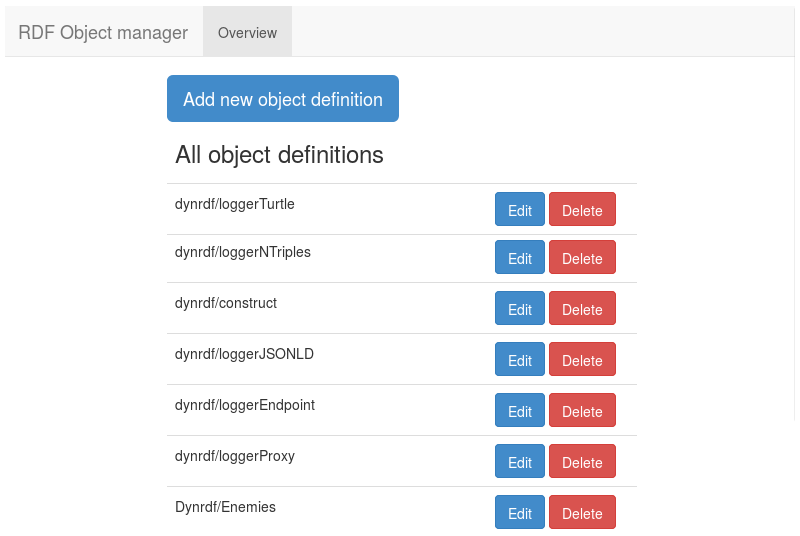
\includegraphics[width=\textwidth]{web_overview}
 	\caption[Přehled definic ve webové aplikaci - hlavní stránka]{Přehled definic ve webové aplikaci - hlavní stránka}\label{web_overview}		
  \end{figure}
    
    \subsection{Vytvoření nové definice}
    Po kliknutí na tlačítko \uv{Add new object definition} je uživatel přesměrován na formulář pro založení nové definice. Tento formulář je zobrazen na obrázku
    \ref{web_create}.
    Uživatel zde nastavuje všechny atributy pro generování objektů.
    Ke každému atributu je na stránce také k dispozici nápověda, která se uživateli zobrazí po kliknutí na obrázek otazníku.
    Těmito atributy jsou:
    \begin{itemize}
     \item Název definice a skupina
      \subitem Název a skupina tvoří dohromady celé jméno definice ve formátu \textit{<skupina>/<název>}. Toto označení definice musí být v celém systému 
      unikátní. Uživatel může pojmenovat více definic stejným jménem, ale tyto definice musí mít rozdílné skupiny.
      
      Zavedení parametru $skupina$ má také výkonostní důvody, které jsou popsány v kapitole Přístup k objektům \ref{obj_access}.
      
      \item Regulární výraz
	\subitem Konkrétní definice jsou v systému identifikovány regulárním výrazem. Při požadavku klienta na konkrétní objekt se server pokouší najít v 
	definicích regulární výraz, který požadované URL adrese odpovídá. Pokud tuto definici nalezne, tak podle ní vygeneruje výsledný objekt.
	
	Například regulární výraz \uv{\textbackslash /objects\textbackslash /time} popisuje URL \url{http://company.com/objects/time/year/2016}.
	Pokud požadavek klienta obsahuje tuto URL adresu a v systému existuje definice s daným regulárním výrazem, je výsledný objekt vygenerován
	dle této definice.
	
	
      \item Priorita
	\subitem Tento atribut určuje pořadí definic, ve kterém se bude systém snažit najít odpovídající definici při požadavku klienta. 
	Mezi jednotlivými definicemi může docházet ke konfliktům regulárních výrazů. Tyto výrazy nemusí být stejné, ale mohou popisovat velmi podobné struktury.
	Při nedefinovaném pořadí vyhledávání v definicích může docházet k nalezení shody u špatných definic a tudíž k vygenerování špatného objektu.
	Nastavením správných priorit lze tomuto problému alespoň zčástí předcházet. Definice jsou prohledávány v pořadí od nejvyšší (1) priority po nejmenší.
	
      \item Typ definice
	\subitem Typ definice určuje, jak bude generování objektu probíhat. Aplikace podporuje několik typů definic. Jedná se o RDF serializace (Turtle, JSON-LD, 
	N-Triples a RDF/XML), SPARQL dotazy (lokální Construct, nebo Construct/Describe dotaz na SPARQL endpointu) a typ Proxy, 
	který funguje na principu přeposílání požadavků.
	Všechny tyto typy jsou dále popsány v kapitole Typy definic \ref{def_types}
	
    \item Šablona definice
      \subitem Typ šablony závisí na typu definice. U RDF serializací se jedná o šablonu v konkrétní serializaci, zatímco u SPARQL typů
      se jedná o SPARQL dotaz. V šablonách se mohou využívat placeholdery pro dosazení parametrů z URL adresy. Šablonovací systém včetně formátu je popsán v kapitole
      Šablonovací systém \ref{template_system}. U typu Proxy se tento atribut nevyplňuje.
      
      \item HTML šablona
      \subitem HTML šablona slouží pro zobrazení dat o objektu v HTML formátu při požadavku z webových prohlížečů. Stejně jako u šablony definice se mohou využívat
      placeholdery pro dosazení parametrů z URL adresy.	
	
    \end{itemize}
    \begin{figure}\centering
 	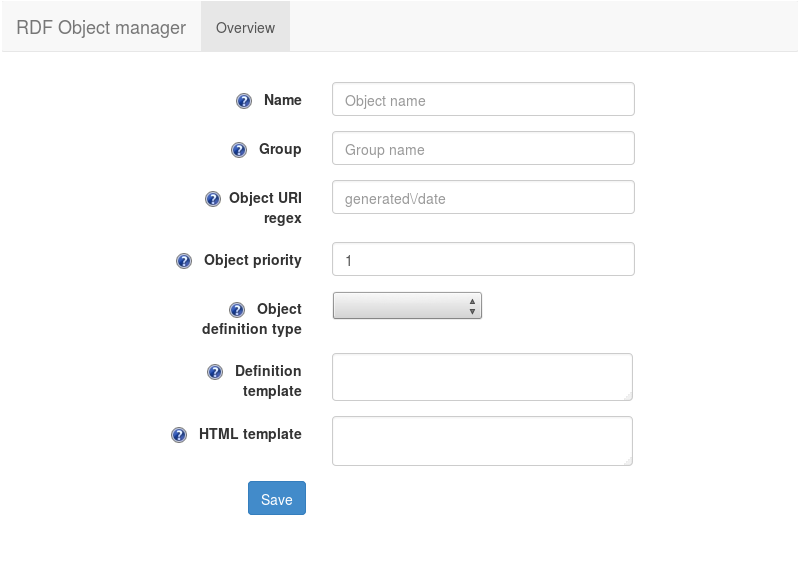
\includegraphics[width=\textwidth]{web_create}
 	\caption[Formulář pro založení a editaci definice]{Formulář pro založení a editaci definice}\label{web_create}		
  \end{figure}
    
    \subsection{Editace definic}
    Po kliknutí na tlačítko \uv{View} v přehledu definic je uživatel přesměrován na informace o dané definici.
    Tyto informace jsou přístupné v editovatelném formuláři. Tento formulář je strukturou totožný s 
    formulářem pro tvorbu nových definic.
    
    \subsection{Mazání definic}
    Uživatel může smazat konkrétní definici přes webovou aplikaci kliknutím na tlačítka \uv{Delete} a následním potvrzením.
    Smazanou definici již nejde žádným způsobem znovu obnovit.    
    
    \section{Typy definic}\label{def_types}
    U každé následující definice jsou uvedeny příklady pro stejný typ objektu - logovací systém, který je také
    dostupný v příloze v ukázkových objektech. Jedná se o objekt logované informace, který očekává URL o délce deseti parametrů. Z URL požadavku
    na tento objekt jsou dosazeny atributy: ID logu, datum, zpráva a název třídy.
      
    \subsection{RDF serializace}
     Tento typ se dělí na definice dle konkrétních serializací - Turtle, N-Triples, RDF/XML a JSON-LD. Uživatel do šablony objektu dosadí
     již serializovaná data a na místech, kam se mají dosadit parametry z URL adresy vytvoři placeholdery.
     Následující příklad šablony je typu Turtle:
     
     \begin{lstlisting}[language=C, basicstyle=\small,]
@base <[@0, "^([^/]*\/[^/]*\/[^/]*\/[^/]*\/[^/]*)\/"]> .
@prefix rlog: 
<http://persistence.unileipzig.org/nlp2rdf/ontologies/rlog#>.
@prefix xsd: <http://www.w3.org/2001/XMLSchema#> .

<#[@6]> # log id 
	a rlog:Entry ;
  	rlog:level rlog:WARN ;
	rlog:date "[@7]T[@8]Z"^^xsd:dateTime ;
	rlog:className "[@9]";
	rlog:message "[@10]".
\end{lstlisting}
 
    \subsection{SPARQL Construct}
      Šablonou pro tento typ je SPARQL Construct dotaz, kde se jednotlivé parametry mohou například vytvářet pomocí funkce \textit{BIND()}.
      Tento typ definice díky jazyku 
      SPARQL doplňuje RDF serializace o další funkcionality tohoto dotazovacího jazyka.
      Příklad stejného objektu pro SPARQL dotaz:
      
           \begin{lstlisting}[language=C, basicstyle=\small,]
PREFIX rlog:  
<http://persistence.unileipzig.org/nlp2rdf/ontologies/rlog#>
PREFIX xsd:   <http://www.w3.org/2001/XMLSchema#>
CONSTRUCT { 
?res a rlog:Entry ;
  	rlog:level rlog:WARN ;
	rlog:date "[@7]T[@8]Z"^^xsd:dateTime ;
	rlog:className "[@9]";
	rlog:message "[@10]".
  }
WHERE {
    BIND (URI('[@0, 
    "^([^/]*\/[^/]*\/[^/]*\/[^/]*\/[^/]*)\/"]#[@6]')
    AS ?res) }
\end{lstlisting}
      
      
    \subsection{SPARQL Endpoint}
      Tento typ je rozšířením typu SPARQL Construct. Dotaz je spouštěn vzdáleně na SPARQL endpointu, přes který je možné přistupovat k datasetům které jsou
      na endpointu dostupné. Tento typ podporuje dva typy dotazů - Construct a Describe a narozdíl od předchozího typu může obsahovat komplikovanější
      dotazy právě nad zmíněnými datasety.
      
    \subsection{Proxy}
      Uživatel může nakonfigurovat přeposílání požadavků na jiný server, který poskytuje také data v RDF serializacích. Jedná se o případy, kdy uživateli
      nestačí výše zmíněné typy a potřebuje nějaký sofistikovanější generátor pro konkrétní objekt. Server tedy pouze přeposílá požadavek a výsledná
      data poté serializuje dle požadavku klienta.
    
    
    
    \section{Šablonovací systém}\label{template_system}
    // TODO
    
    \section{Přístup k objektům}\label{obj_access}
    // TODO
    
  \section{Instalace serveru}
  
  \subsection{Systémové požadavky}
  \begin{itemize}
   \item Webový server pro webové aplikace v Javě Tomcat nebo Glassfish
   \item Java 1.8
  \end{itemize}
    
  \subsection{Instalace přes webový archiv}
  Instalace serveru přes přiložený webový archiv je nejjednodušší variantou. Pro správný chod celého serveru je potřeba před nasazením nastavit konfiguraci serveru.
  Celá instalace má následující kroky:
  \begin{itemize}
   \item Ve filesystému založte adresář pro definice objektů a zajistěte práva pro čtení i zápis pro webový server
   \item Nakopírujte do tohoto adresáře ukázkové objekty z adresáře $objects$
   \item Otevřte přiložený soubor $dynrdf.war$ v libovolném manažeru archivů
   \item V archivu otevřte soubor $/WEB-INF/classes/config.properties$ dle obrázku \ref{config} a nastavte zde parametr $ObjectsPath$ aby směřoval na 
   adresář s definicemi. Parametry $ObjectBaseUrl$ a $ObjectRDFS$ se používají při ukládání definic do Turtle formátu a měly by směřovat na základní URL serveru
   a URL s přístupem ke schématu definic (RDFS).
   \item V archivu otevřte soubor $/WEB-INF/classes/log4j.properties$ a nastavte zde parametr $log4j.appender.file.File$ na cestu, kam chcete ukládat logy.
   Můžeté také změnit styl logování, případně změnit i typ logování z $DEBUG$ na jiný typ prostředí.
   \item Uložte upravený webový archiv
   \item Nahrajte soubor $dynrdf.war$ na aplikační server. Na serveru Tomcat pomocí formuláře pro nahrátí na obrázku \ref{tomcat_deploy}.
  \end{itemize}

      \begin{figure}\centering
 	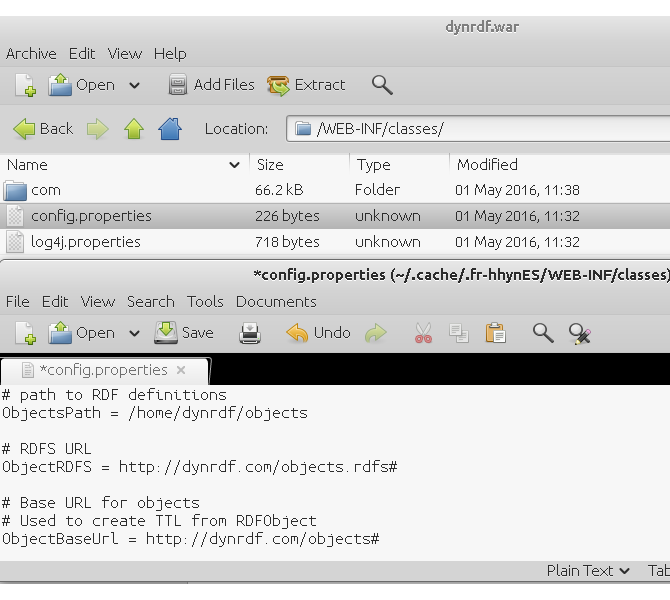
\includegraphics[width=\textwidth]{config}
 	\caption[Nastavení parametrů v konfiguračním souboru]{Nastavení parametrů v konfiguračním souboru}\label{config}		
  \end{figure}
  
        \begin{figure}\centering
 	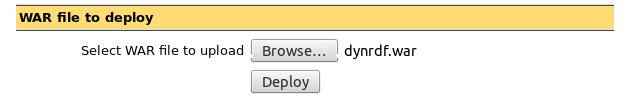
\includegraphics[width=\textwidth]{tomcat_deploy}
 	\caption[Nahrátí webového archivu na server Tomcat]{Nahrátí webového archivu na server Tomcat (adresa /manager/html) - vyberte war soubor z adresáře a klikněte na deploy}\label{tomcat_deploy}		
  \end{figure}
  

  
  \subsection{Instalace ze zdrojových kódů}
  Pro instalaci ze zdrojových kódu je potřba mít nainstalovaný program Maven.
  Instalace má tyto kroky:
   \begin{itemize}
   \item Nastavte parametry v konfiguračních souborech podobně jako při instalaci z připraveného war souboru. Konfigurační soubory se
   nacházejí ve složce $src/main/resources$.
   \item Vytvořte ze zdrojových kódů webový archiv pomocí příkazu $mvn \ package$ v kořenu zdrojových kódu (tam kde je uložen soubor $pom.xml$).
   \item Webový archiv, který najdete ve složce $target$, která se po provedení příkazu vytvořila, nahrajte na aplikační server stejně jako 
   v případě instalace serveru z war souboru.
  \end{itemize}

  
  
\begin{conclusion}
Cílem této práce bylo navrhnout, implementovat a otestovat webový server pro poskytování dynamicky generovaných objektů v RDF formátech.
Serveru byly určeny požadavky zadáním této práce a také dalšími v průběhu tvorby této práce. Dalšími požadavky se zabývala převážně analytická část.

Všechny tyto požadavky a cíle byly splněny.
Návrhu předcházela analýza účelu aplikace a podobných řešení. Závěrem této analýzy bylo, že neexistuje žádný server, který by poskytoval funkce
implementovaného serveru. To dává této práci šanci být využívanou ve velkém měřítku.

Na základě analýzy byl proveden návrh celého systému a následně jeho implementace. Bylo použito několik pokročilých technologií jak z oboru Linked Data,
tak i z pohledu implementace.

Testování proběhlo na několika úrovních. Základem byly unit testy netriviálních metod tříd, na které navázaly komplexnější testy celé aplikace.
Server byl také otestován na výkon.


Mně osobně přinesla tato práce mnoho nových zkušeností a znalostí. Jedná se převážně o obor Linked Data, který mne velice zaujal a plánuji se mu i dále věnovat.
Z pohledu implementace se jednalo o zatím největší aplikaci v Javě, kterou jsem programoval. Vyzkoušel jsem si práci s velkým množstvím kvalitních knihoven,
které se ve světě velmi často používají. Z pohledu testování jsem si osvojil nové techniky testování aplikací v Javě, především těch webových. Také jsem se poprvé
věnoval testování výkonu webové aplikace.
Ve vývoji této práce plánuji i nadále pokračovat.


S využitím této práce se počítá pro datasety otevřené datové infrastruktury opendata.cz.		

\end{conclusion}

\bibliographystyle{csn690}
\bibliography{mybibliographyfile}

\appendix

\chapter{Seznam použitých zkratek}
% \printglossaries
\begin{description}
	\item[RDF] Resource description framework
	\item[URI] Uniform Resource Identifier
	\item[URL] Uniform Resource Locator
	\item[HTTP] Hypertext Transfer Protocol
	\item[WWW] World Wide Web
	\item[HTML] HyperText Markup Language
	\item[SPARQL] Protocol and RDF Query Language
	\item[API] Application program interface
	\item[CRUD] Create, read, update and delete
	\item[IP] Internet Protocol 
	\item[MVC] Model–view–controller
	\item[JSON] JavaScript Object Notation
\end{description}



\chapter{Obsah přiloženého CD}
\begin{figure}[H]
	\dirtree{%
		.1 readme.txt\DTcomment{stručný popis obsahu CD}.
		.1 install.txt\DTcomment{instalační pokyny pro nasazení war souboru}.
		.1 dynrdf.war\DTcomment{war soubor pro deploy na server}.
		.1 objects\DTcomment{adresář s ukázkovými objekty}.
		.1 testObjects\DTcomment{adresář s objekty pro testování}.
		.1 img \DTcomment{adresář s obrázky administrace a požadavku na objekt}.
		.1 src.
		.2 impl\DTcomment{zdrojové kódy implementace}.
		.2 thesis\DTcomment{zdrojová forma práce ve formátu \LaTeX{}}.
		.1 text\DTcomment{text práce}.
		.2 thesis.pdf\DTcomment{text práce ve formátu PDF}.
	}
\end{figure}

\end{document}
